
In spline interpolation\cite{Boor1981}, as in the linear case, we will define a piecewise
function, but employing polynomials to join the different points known.
The main advantage of using splines of order $n$, i.e., using polynomial of
order $n$ in the different intervals, is that we will not only obtain continuous
functions, as in the linear case, but we will also obtain functions
$\mathcal{C}^{n-1}[a,b]$. This fact will be crucial in FDA, because we will need
to use derivatives in many phases of the analysis.

\begin{figure}[Example of spline interpolation]{FIG:SPLINE}{Example of spline interpolation}
	\subfigure[SBFIG:SPLINE1]{Spline interpolation}{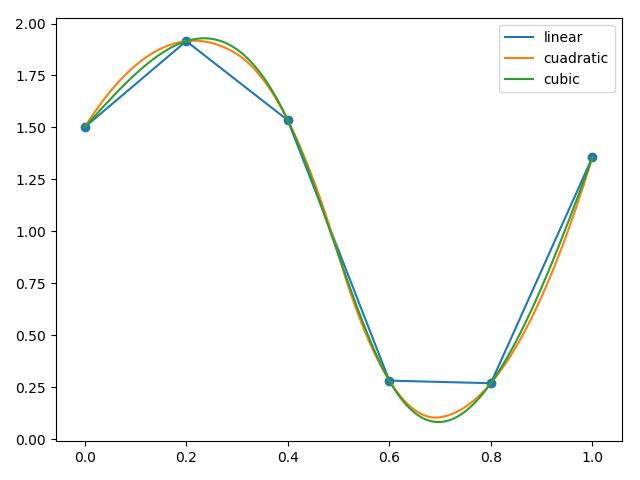
\includegraphics[width=7.5cm]{spline-interpolation}} \quad
	\subfigure[SBFIG:SPLINE2]{First derivatives}{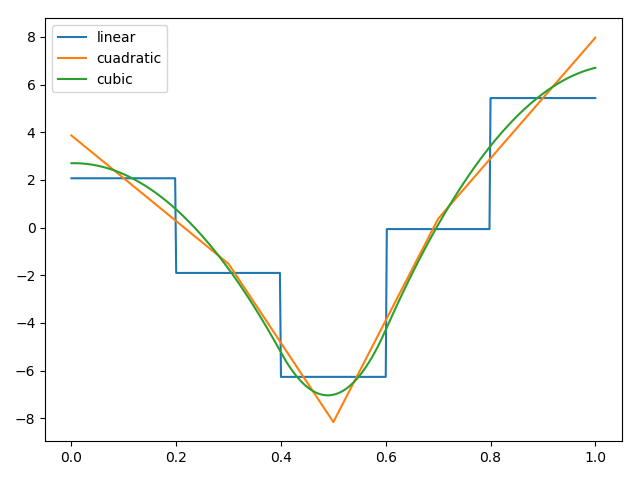
\includegraphics[width=7.5cm]{spline-derivatives-interpolation}}
\end{figure}

To achieve this, we will have to match the values of the derivatives of the
adjacent splines in the interpolation knots. If we denote by
$p_k(t)=\sum_{j=0}^n c_{jk} t^k$ to the spline defined in the region
$[t_{k-1}, t_{k}]$, during the calculation of the coefficients $c_{jk}$, we must
impose the restriction $p_{k}^{(d)}(t_k) = p_{k+1}^{(d)}$ for \\ $d=1, \dots, n-1$.
For this purpose, we will define a linear system of equations which will be
solved iteratively. Figure \ref{SBFIG:SPLINE1} shows the result of interpolate a
temporal series using splines of different orders, and the first derivatives of
these splines, which are splines of order $n-1$ due to the derivation of the
polynomials.

\begin{figure}[Interpolation of surface]{FIG:BISPLINE}{Interpolation of surface with bicubic splines}
	\subfigure[SBFIG:BISPLINE1]{Surface interpolated}{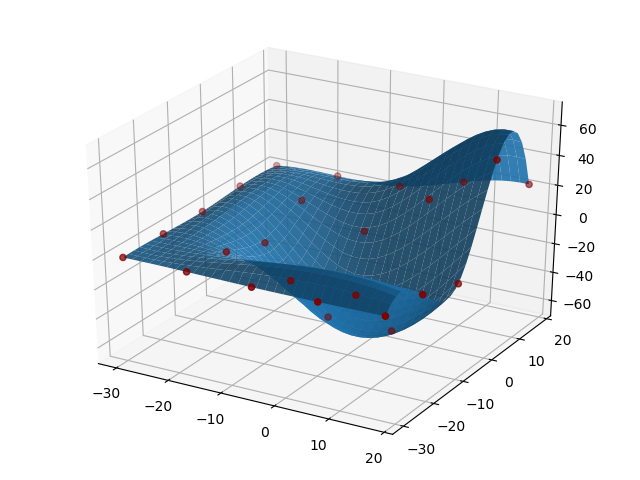
\includegraphics[width=7.5cm]{surface-bicubic}} \quad
	\subfigure[SBFIG:BISPLINE2]{Partial derivative $\partial_x$}{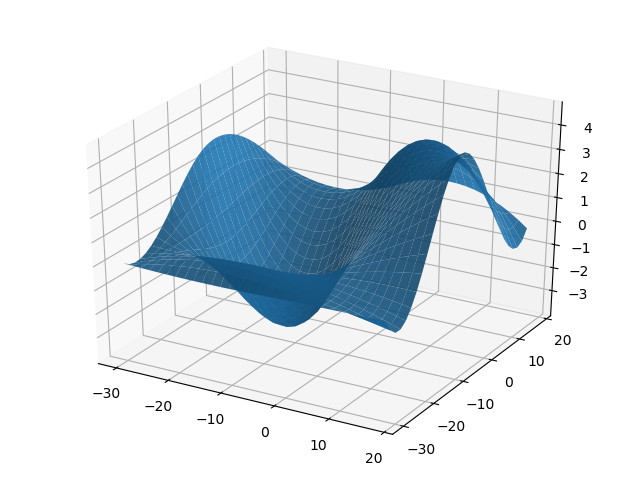
\includegraphics[width=7.5cm]{surface-bicubic-dx}}
\end{figure}

We can extend spline interpolation for multivariate functions, such as surfaces,
where bivariate splines will be used. In this case, it is used triangulation
to calculate the regions in which the polynomials will be defined, which will
be of the form $p(x, y) = \sum_{0 \le i + j \le n} c_{i,j}x^i y^j$.
In the figure \ref{SBFIG:BISPLINE1} it is shown the result of the
interpolation of a surface using bicubic splines and the partial derivative,
respect to $x$, of the surface.
